\documentclass[12pt,a4paper]{report}

% ----------------------------------------------------------------------
% PACKAGES AND CONFIGURATION
% ----------------------------------------------------------------------
\usepackage[utf8]{inputenc}
\usepackage[T1]{fontenc}
\usepackage{mathptmx}              % Times New Roman-compatible font (text + math)
\usepackage[margin=1in]{geometry}
\usepackage{setspace}
\onehalfspacing
\usepackage{graphicx}
\usepackage{amsmath,amssymb}
\usepackage{array}
\usepackage{tabularx}
\usepackage{xltabular}
\usepackage{longtable}
\usepackage{ragged2e}
\usepackage[table]{xcolor}
\usepackage{enumitem}
\usepackage{titlesec}
\usepackage{fancyhdr}
\usepackage{float}
\usepackage{caption}
\usepackage{cite}
\usepackage[hidelinks,colorlinks=true,linkcolor=black,citecolor=black,urlcolor=black]{hyperref}
\usepackage[none]{hyphenat}
\hyphenpenalty=10000
\exhyphenpenalty=10000
\sloppy

% ---------------- TABLE STYLE ----------------
\renewcommand{\arraystretch}{1.3}
\setlength{\tabcolsep}{4pt}
\newcolumntype{L}[1]{>{\RaggedRight\arraybackslash}p{#1}}
\newcolumntype{C}[1]{>{\Centering\arraybackslash}p{#1}}
\newcolumntype{Y}{>{\RaggedRight\arraybackslash}X}
\newcommand{\hdrrow}{\rowcolor{gray!20}}

% Table captions strictly ABOVE, figure captions strictly BELOW
\captionsetup[table]{position=above, font=small, labelfont=bf, skip=6pt}
\captionsetup[figure]{position=below, font=small, labelfont=bf, skip=6pt}

% ---------------- HEADER / FOOTER ----------------
\setlength{\headheight}{14pt}

% Default style for regular body pages: running header with rule, full department footer with rule
\fancyhf{}
\fancyhead[L]{\small AI-Driven Convective Nowcasting}
\fancyhead[R]{\small 2026 - 27}
\fancyfoot[L]{\scriptsize Department of Master of Computer Applications (MCA), VCET, Puttur}
\fancyfoot[R]{\small Page \thepage}
\renewcommand{\headrulewidth}{0.4pt}
\renewcommand{\footrulewidth}{0.4pt}
\pagestyle{fancy}

% Plain style for Chapter opening pages: completely empty
\fancypagestyle{plain}{
  \fancyhf{}
  \renewcommand{\headrulewidth}{0pt}
  \renewcommand{\footrulewidth}{0pt}
}

% ---------------- HEADINGS (LEFT-ALIGNED) ----------------
\titleformat{\chapter}[display]
  {\fontsize{16pt}{20pt}\selectfont\bfseries}
  {\raggedright\chaptertitlename\ \thechapter}
  {8pt}
  {\centering\fontsize{16pt}{20pt}\selectfont\bfseries}
\titlespacing*{\chapter}{0pt}{10pt}{22pt}
\assignpagestyle{\chapter}{empty}

\titleformat{\section}
  {\fontsize{14pt}{18pt}\selectfont\bfseries\raggedright}{\thesection}{1em}{}

\titleformat{\subsection}
  {\fontsize{14pt}{18pt}\selectfont\bfseries\raggedright}{\thesubsection}{1em}{}

% ----------------------------------------------------------------------
% DOCUMENT STARTS (Directly from Abstract)
% ----------------------------------------------------------------------
\begin{document}

% ----------------------------------------------------------------------
% ABSTRACT (PAGE i)
% ----------------------------------------------------------------------
\pagenumbering{roman}
\setcounter{page}{1}
\thispagestyle{empty}

\begin{center}
{\fontsize{15pt}{19pt}\selectfont \textbf{AI-DRIVEN CONVECTIVE WEATHER AND THUNDERSTORM NOWCASTING SYSTEM FOR KARNATAKA USING ATMOSPHERIC THERMODYNAMICS AND GENERATIVE AI}}\\[0.5cm]
{\fontsize{14pt}{18pt}\selectfont \textbf{ABSTRACT}}\\[0.5cm]
\end{center}

\noindent An intelligent, physics-informed convective weather and thunderstorm nowcasting system is developed to deliver high-precision, short-term ($0$--$90$ minutes) meteorological predictions across Karnataka, with specialized calibration for the Western Ghats and coastal regions. Tropical thunderstorms, convective lightning discharges, and localized downbursts pose severe risks to agriculture, transport, and public safety. Conventional Numerical Weather Prediction models suffer from update latency ($3$--$6$ hours) and coarse resolutions that fail to resolve fast-evolving convective cells igniting within $30$ to $60$ minutes. The developed framework bridges this gap by unifying a 27-year historical Karnataka climatological dataset ($9,862$ verified daily records from 2000 to 2027), real-time atmospheric telemetry, and multimodal generative reasoning via the Google Gemini API. The system implements a 62-feature atmospheric pipeline computing continuous thermodynamic indices, including Dew Point Depression, Vapor Pressure Deficit, and Equivalent Potential Temperature to suppress nocturnal false alarms. A soft-voting Gradient Boosted Decision Tree ensemble (LightGBM, XGBoost, HistGradientBoosting) achieves 91.2\% holdout accuracy, calibrated alongside climatological priors. Integrated Gemini AI reasoning translates complex predictive distributions into calibrated convective risk probabilities, a 3-step timeline progression ($+30$m, $+60$m, $+90$m), and plain-language domain advisories for agriculture, transit, and public safety. An interactive Leaflet.js Doppler radar interface delivers accessible, low-latency decision support for regional disaster preparedness.

\vspace{0.8cm}
\noindent \textbf{Keywords:} Convective Weather Nowcasting, Thunderstorm Prediction, Atmospheric Thermodynamics, Gradient Boosted Trees, Google Gemini API, S-Band Doppler Radar, Western Ghats Microclimates, Dew Point Depression.
\newpage
\tableofcontents
\thispagestyle{empty}

\newpage
\listoffigures
\thispagestyle{empty}

\newpage
\listoftables
\thispagestyle{empty}

% ----------------------------------------------------------------------
% CHAPTER 1: INTRODUCTION
% ----------------------------------------------------------------------
\newpage
\pagenumbering{arabic}
\setcounter{page}{1}
\pagestyle{fancy}

\chapter{Introduction}
\thispagestyle{empty}

% \section{Background}
Severe thunderstorms, heavy rainfall in small areas, and lightning are dangerous weather events that can cause serious damage in tropical regions. In Karnataka, the Arabian Sea coast and the high mountains of the Western Ghats create conditions that can lead to the rapid formation of thunderstorms. During the pre-monsoon season (March to May) and post-monsoon season (October to November), strong sunlight heats the ground, while moist air from the sea helps storms develop quickly.

Nowcasting involves analyzing real-time atmospheric observations to forecast imminent convective activity within an immediate temporal window. The developed system focuses specifically on predicting severe thunderstorms and lightning strikes up to 90 minutes in advance. In areas such as Dakshina Kannada, Udupi, and the Malenadu hills, storms can form quickly and cause lightning, sudden flooding, and strong winds before regular weather forecasts detect them.

To address this problem, the proposed system uses machine learning and generative AI to analyze live weather data, past weather records, and Doppler radar information. It aims to predict local thunderstorms and lightning quickly and provide timely warnings to help people prepare for dangerous weather.

\section{Problem Statement}
Weather forecasts in Karnataka mainly use numerical weather prediction models run by national weather agencies. These models are useful for predicting general weather conditions 24 to 72 hours in advance, but they may not predict local thunderstorms accurately within a short time. They may also take 3 to 6 hours to update and may miss small storms that develop and disappear within 30 to 60 minutes, especially in the narrow valleys of the Western Ghats.
Some weather applications use fixed rules to predict storms. However, high humidity at night in coastal areas and towns such as Puttur and Bantwal may sometimes be wrongly identified as a sign of a thunderstorm. This can lead to unnecessary warnings and confusion. Also, live weather station data is not always compared with long-term weather records, which can cause sudden and unreliable changes in predictions.
Many existing weather websites display numbers and simple alerts without explaining what people should do. As a result, farmers, transport operators, and disaster management teams may not get the clear information they need to prepare for severe weather.
To overcome these limitations, the developed system establishes an integrated, real-time nowcasting platform combining live station telemetry, historical climate records, machine learning models, and AI-generated weather reports. It provides localized thunderstorm and lightning predictions alongside actionable warnings to support frontline decision-making.

\section{Objectives}
The core objectives of the proposed nowcasting system are:
\begin{itemize}[leftmargin=1.2em, itemsep=3pt, topsep=2pt]
    \item \textbf{To develop an AI/ML-based system for short-term thunderstorm and lightning nowcasting:} \\
    To provide real-time convective storm and lightning alerts within a $0$ to $90$-minute prediction window.

    \item \textbf{To process a 27-year regional climatological dataset and build a 62-feature atmospheric physics pipeline:} \\
    To combine 27 years of historical Karnataka weather data ($9,862$ records) with thermodynamic features (DPD, VPD) to prevent nighttime false alarms.

    \item \textbf{To develop and evaluate machine learning and deep learning models for 30, 60, and 90-minute predictions:} \\
    To train tree ensembles and evaluate calibrated storm risk probabilities at $+30$, $+60$, and $+90$-minute intervals.

    \item \textbf{To deploy an interactive decision dashboard with Gemini Generative AI bulletins and dynamic radar visualization:} \\
    To integrate Google Gemini AI for plain-language sector advisories alongside an interactive Doppler radar map and taluk micro-zones.
\end{itemize}

\section{Scope}
The system covers the whole state of Karnataka, from 11.5°N to 18.6°N latitude and 74.0°E to 78.6°E longitude. It is designed to work with the weather conditions of three regions: Coastal Karnataka, the Western Ghats, and Interior Karnataka. The system collects live weather data and uses 62 weather features and multiple machine learning models to predict thunderstorms and lightning. It also creates weather reports automatically and uses interactive S-band Doppler radar data to predict storms in areas within Karnataka.

\section{Motivation}
Thunderstorms and lightning inflict severe damage on standing crops, infrastructure, and human life across Karnataka. The developed nowcasting platform provides an accessible, high-precision warning system that forecasts convective events up to 90 minutes in advance, enabling farmers, transport operators, and local administrations to execute timely precautionary measures.

\section{Chapter Summary}
The introductory chapter established the operational background, problem statement, core objectives, geographical scope, and motivation for AI-driven convective storm nowcasting across Karnataka. Severe weather vulnerabilities across the coastal belt and the Western Ghats were analyzed, emphasizing the critical limitations of conventional numerical weather prediction systems. The overarching goal of delivering rapid, physics-grounded $0$--$90$ minute nowcasts was formulated, providing the foundation for the scientific literature review.

% ----------------------------------------------------------------------
% CHAPTER 2: LITERATURE REVIEW
% ----------------------------------------------------------------------
\chapter{Literature Review}
\thispagestyle{empty}

The literature review investigates recent scientific advancements and methodologies in atmospheric physics, remote sensing, and artificial intelligence for convective storm and lightning nowcasting. Severe convective storms evolve rapidly within $30$ to $90$ minutes, making early detection and localized warning difficult for traditional numerical weather prediction models. To address these limitations, contemporary researchers have explored diverse computational paradigms. For instance, Tian et al. \cite{tian2026dual} formulated dual-weighted loss functions to counter extreme spatial imbalance between quiescent clear skies and active storm cells. Chen et al. \cite{chen2026clka} demonstrated the utility of coupling neural networks with Kolmogorov-Arnold Networks (KAN) to map physical atmospheric sounding profiles to lightning flash rates. In operational evaluations across northern India, Kumar et al. \cite{kumar2026enhancing} showed that gradient-boosted decision tree ensembles consistently outperform deep neural networks on tabular meteorological datasets. In satellite meteorology, Sharma et al. \cite{sharma2025insat} utilized Indian INSAT-3D thermal infrared channels to detect pre-convective cloud clusters before surface rainfall begins, while Rayudu et al. \cite{rayudu2025prediction} evaluated deep recurrent architectures on Doppler radar reflectivity grids to model cell translation across southern India. In addition, empirical radar investigations over Karnataka by Toropova et al. \cite{toropova2022characteristics} highlighted the strong connection between radar reflectivity cores, cloud heights, and post-monsoon electrical activity. Reviewing these foundational studies provides valuable technical insights into feature selection, radar processing, and ensemble modeling, while identifying critical gaps in localized thermodynamic grounding that motivate the proposed system.

\section{Existing Studies}
Recent investigations in convective nowcasting and severe storm modeling have achieved significant breakthroughs through specialized loss formulations, deep physical soundings, and machine learning ensembles. Addressing the extreme spatial imbalance between quiescent background regions and active storm cores, Tian et al. \cite{tian2026dual} formulated dual-weighted loss functions that penalize missed detections in high-reflectivity convective centers. Incorporating non-linear functional representations, Chen et al. \cite{chen2026clka} coupled convolutional recurrent networks with Kolmogorov-Arnold Networks (KAN) to map physical sounding profiles to total lightning flash rates. Operational ensemble evaluations across northern India by Kumar et al. \cite{kumar2026enhancing} demonstrated that Gradient Boosted Decision Tree (GBDT) architectures (XGBoost and LightGBM) consistently outperform deep neural networks on tabular sounding datasets. Remote sensing pre-convective indicators were advanced by Wang et al. \cite{wang2026infrared}, who demonstrated that rapid brightness temperature drops in geostationary split-window infrared channels signal cloud-top glaciation and imminent lightning. To prioritize developing convective cores over dissipating anvil debris, Li et al. \cite{li2026nowcasting} integrated spatial attention mechanisms into Conv-GRU backbones for cloud-to-ground flash density mapping. Establishing direct physical reflectivity warning thresholds, Li et al. \cite{li2026correlation} verified that $40$~dBZ radar echo volumes extending above the freezing level provide unambiguous operational precursors of surface lightning discharges.

Multimodal data fusion and remote sensing validation have significantly expanded operational observation coverage across diverse geographical domains. Deploying self-supervised representation learning, Zhang et al. \cite{zhang2025lightning} fused optical satellite imagery with high-frequency lightning telemetry to track convective storm translation. Ground-based remote sensing validation across the Indian subcontinent by Ghosh et al. \cite{ghosh2025assessment} established that the Indian Lightning Location Network (ILLN) achieves detection efficiencies exceeding 88\%, while highlighting pronounced terrain-induced signal attenuation across the Western Ghats. In satellite meteorology, Sharma et al. \cite{sharma2025insat} leveraged Indian INSAT-3D thermal infrared channels to identify pre-convective cloud clusters before surface precipitation begins. Focusing on southern India, Rayudu et al. \cite{rayudu2025prediction} evaluated deep recurrent architectures (ConvLSTM and PredRNN) on Doppler Weather Radar (DWR) reflectivity grids to model localized cell translation and decay.

Polarimetric radar capabilities and multi-source data fusion have further advanced convective warning horizons and hydrometeor classification. Rombeek et al. \cite{rombeek2024exploiting} proved that dual-polarization radar parameters ($Z_{DR}, K_{DP}$) substantially enhance deep learning hydrometeor classification during thunderstorm intensification. Demonstrating the vital necessity of boundary-layer surface physics, Kim et al. \cite{kim2024improvements} established that fusing automated weather station (AWS) surface factors---specifically dry-bulb temperature, relative humidity, and pressure---with radar rain rate significantly slows nowcast degradation beyond 30 minutes. In operational US meteorology, Cintineo et al. \cite{cintineo2024probsevere} established NOAA's ProbSevere v3 framework, demonstrating that multi-sensor GBDT data fusion combining radar, satellite, and numerical model fields provides superior calibrated severe storm probabilities. Analyzing seasonal lightning dynamics across Indian climate zones, Soni et al. \cite{soni2023machine} demonstrated the strong geographic dependency of electrical discharges on Convective Available Potential Energy (CAPE) and total precipitable water. Specifically within Karnataka, Toropova et al. \cite{toropova2022characteristics} conducted an extensive empirical radar investigation over Gadag ($15^\circ\text{N}$), analyzing more than 2,500 convective clouds and 5,000 electrical discharges to prove that maximum radar reflectivity ($Z_{\max}$), cloud-top height, and lightning frequency surge during post-monsoon transition periods.

Spatiotemporal recurrent architectures, multi-hazard data fusion, and aerosol interactions have further expanded the theoretical and empirical frontiers of convective storm prediction. Leinonen et al. \cite{leinonen2022seamless, leinonen2022nowcasting, leinonen2023multihazard} demonstrated that recurrent-convolutional networks and multi-hazard fusion combining radar, satellite, and lightning observations enable seamless probabilistic prediction of thunderstorm initiation, motion, and severity. In the context of operational numerical prediction over India, Prasad et al. \cite{prasad2023impact} established that assimilating Indian Doppler radar reflectivity and lightning strike records significantly enhances short-range quantitative precipitation forecasts for severe rain events. To overcome motion blur and deformation in deep extrapolation, Luo et al. \cite{luo2021pfst} formulated the PFST-LSTM model, which incorporates physical pseudoflow representations into spatiotemporal memory cells for convective nowcasting. Exploring microphysical interactions, Song et al. \cite{song2023lightning} revealed that coupling aerosol optical depth with geostationary satellite imagery within machine learning pipelines substantially improves flash rate prediction. Sensor network analytics and adversarial learning were advanced by Sibolla et al. \cite{sibolla2021determining}, who developed real-time spatial clustering methods for sensor-based lightning strike monitoring, and Lu et al. \cite{lu2023mcgln}, who developed the MCGLN ConvLSTM-GAN framework for multi-source spatiotemporal lightning nowcasting. Furthermore, Goyal et al. \cite{goyal2017satellite} pioneered satellite-based nowcasting techniques over the Indian region using infrared brightness temperature thresholds, while Le and Vargas \cite{le2024autocorrelated} introduced autocorrelated conditioned Latin hypercube methods to optimize spatial and temporal sampling for geophysical prediction.

Atmospheric instability and convective available energy have historically formed the bedrock of operational thunderstorm forecasting, yet integrating vertical sounding dynamics into real-time algorithms remains a complex challenge. Severe convective storms in the tropics depend heavily on moisture availability in the lower planetary boundary layer and strong diurnal surface heating. While conventional soundings provide diagnostic indices such as Convective Available Potential Energy (CAPE), Convective Inhibition (CIN), Lifted Index (LI), and the K-Index, their coarse temporal resolution (typically 12-hourly rawinsonde launches) prevents their direct application to sub-hourly nowcasting. Recent machine learning approaches attempt to infer vertical instability from surface meteorological networks; however, without continuous thermodynamic metrics such as Dew Point Depression (DPD) and Vapor Pressure Deficit (VPD), models frequently generate false alarms during high-humidity periods. Establishing deterministic boundary-layer saturation constraints is essential to distinguish between non-precipitating stratiform mist and active convective updrafts.

A critical architectural divergence in modern nowcasting literature lies between deep spatiotemporal computer vision networks and gradient-boosted decision trees (GBDTs). Deep architectures, including ConvLSTM, TrajGRU, and UNet-based models, excel at spatial motion extrapolation by treating consecutive radar reflectivity grids or satellite imagery channels as video frames. However, these computer-vision methods frequently suffer from progressive blur and loss of high-reflectivity convective peaks beyond a 30-minute lead time, while requiring substantial GPU acceleration that renders local edge deployment impractical. In contrast, tree ensemble architectures such as LightGBM, XGBoost, and CatBoost operate directly on feature-engineered tabular vectors encompassing surface telemetry, thermodynamic soundings, multi-level pressure tendencies, and historical climatological baselines. Studies demonstrate that when supplied with physically derived variables (such as dew point depression, wet-bulb temperature, and solar insolation weighting), GBDTs achieve comparable or superior classification accuracy with sub-second inference latencies on commodity multi-core processors.

Beyond raw numerical prediction and risk probability scores, the communicative gap between meteorological warning systems and operational stakeholders represents a crucial frontier in convective hazard mitigation. Traditional numerical weather products and automated smartphone applications often present abstract probabilities or generic warning icons that fail to convey actionable risk or localized impacts. For agricultural communities, transportation operators, and district disaster management authorities, effective nowcasts require plain-language contextual bulletins that explain expected storm arrival times, lightning risk tiers, and specific safety advisories. Recent advancements in Natural Language Generation and Large Language Models (LLMs) provide an automated mechanism to synthesize complex multi-sensor telemetry, radar contours, and calibrated machine learning probabilities into coherent, sector-specific meteorological bulletins, bridging the divide between physical forecasting and frontline disaster preparedness. While these twenty-five surveyed studies advance radar tracking, deep learning, and tree ensembles, they either operate at coarse synoptic scales or lack localized thermodynamic grounding and accessible decision-support interfaces for rural tropical regions.

\section{Comparative Summary}
A detailed comparative analysis of key representative surveyed research papers against the proposed nowcasting architecture is presented in Table~\ref{tab:lit_comparison}. The comparison underscores the novelty of the proposed framework in unifying a 27-year regional climatological dataset, continuous thermodynamic boundary-layer indices, gradient boosted tree ensembles, and LLM-driven generative meteorological bulletins within a single localized web platform.

\begingroup
\hyphenpenalty=50
\exhyphenpenalty=50
\sloppy
\begin{xltabular}{\textwidth}{|L{3.8cm}|C{1.3cm}|L{4.3cm}|Y|}
\caption{Comparative Summary of Surveyed Research Papers}\label{tab:lit_comparison} \\
\hline
\hdrrow \textbf{Paper Title} & \textbf{Year} & \textbf{Description} & \textbf{Pros \& Cons} \\ \hline
\endfirsthead
\hline
\hdrrow \textbf{Paper Title} & \textbf{Year} & \textbf{Description} & \textbf{Pros \& Cons} \\ \hline
\endhead
\hline
\endfoot
\hline
\endlastfoot

``A Dual-Weighted Loss Function for Lightning Nowcasting'' \cite{tian2026dual} & 2026 & Dual-weighted loss formulation penalizing false negatives in high-intensity convective storm cores to counter severe pixel imbalance. & \textbf{Pro:} Effectively mitigates severe class imbalance between quiescent and active convective storm pixels. \newline \textbf{Con:} Optimized strictly for loss calculation; requires pairing with external spatiotemporal backbones. \\ \hline
``CLKA-LPO: A CNN-LSTM-KAN Neural Network for Lightning Potential and Flash Rate Prediction Based on Atmospheric Physical Parameters'' \cite{chen2026clka} & 2026 & Deep architecture coupling CNN-LSTM with Kolmogorov-Arnold Networks (KAN) to map sounding parameters to flash density. & \textbf{Pro:} Strong non-linear physical mapping of vertical atmospheric sounding profiles to lightning rates. \newline \textbf{Con:} High theoretical complexity; lacks operational spatial mapping and user-facing decision dashboard. \\ \hline
``Enhancing the Forecasting of Lightning Density Over Northern India: An Ensemble and Deep Learning Models Approach'' \cite{kumar2026enhancing} & 2026 & Comparative evaluation of XGBoost, LightGBM, and Deep Neural Networks on atmospheric soundings across northern India. & \textbf{Pro:} Demonstrates decisive performance superiority of tree ensembles over deep networks on tabular soundings. \newline \textbf{Con:} Operates on broad seasonal and synoptic scales; lacks short-range 0--90 minute nowcast trajectories. \\ \hline
``Infrared Brightness Temperature-Based Indicators for Identifying Thunderstorm Clouds: Insights From FY-4A Satellite Observations'' \cite{wang2026infrared} & 2026 & Split-window infrared brightness temperature difference analysis for early detection of intensifying convective clouds. & \textbf{Pro:} Provides rapid pre-convective cloud-top cooling indicators prior to surface storm initiation. \newline \textbf{Con:} Subject to parallax errors in complex topography; lacks surface boundary-layer thermodynamic checks. \\ \hline
``Nowcasting of Cloud-to-Ground Lightning Location and Frequency Based on a Deep Learning Technique'' \cite{li2026nowcasting} & 2026 & Spatial attention Conv-GRU network predicting lightning strike density grids and discharge frequencies. & \textbf{Pro:} Spatial attention mechanism prioritizes active updrafts over dissipating anvil debris. \newline \textbf{Con:} Heavy computational footprint during multi-step inference; lacks plain-language advisory translation. \\ \hline
``Research on the Correlation Between Meteorological Radar Echo Characteristics and Lightning Warning Technology'' \cite{li2026correlation} & 2026 & Empirical correlation between vertical radar echo volume ($\ge 40$~dBZ above freezing level) and lightning strokes. & \textbf{Pro:} Establishes direct physical radar reflectivity criteria for cloud-to-ground electrical discharge warning. \newline \textbf{Con:} Dependent on high-bandwidth Doppler radar grids; susceptible to beam blockage in mountain valleys. \\ \hline
``A Lightning Augmented Recurrent Nowcasting Model Based on Self-Supervised Learning and Multi-Modal Fusion Method'' \cite{zhang2025lightning} & 2025 & Self-supervised spatiotemporal recurrent framework fusing optical satellite imagery with lightning strike streams. & \textbf{Pro:} Self-supervised pre-training significantly improves convective representation learning. \newline \textbf{Con:} Demands high GPU cluster capacity for inference; not optimized for low-latency web deployment. \\ \hline
``Assessment of the Indian Lightning Location Network (ILLN) Using Ground-Based and Satellite Observations'' \cite{ghosh2025assessment} & 2025 & Empirical assessment of ILLN ground sensor network efficiency against spaceborne optical lightning imagers over India. & \textbf{Pro:} Verifies high cloud-to-ground detection efficiency ($> 88$\%) across Indian landmass. \newline \textbf{Con:} Identifies significant terrain-induced detection attenuation across Western Ghats valleys. \\ \hline
``Leveraging INSAT-3D Indian Geostationary Satellite for Advanced Lightning Detection and Analysis'' \cite{sharma2025insat} & 2025 & Thermal infrared channel tracking on INSAT-3D for detecting rapid cloud-top cooling and convective storm initiation. & \textbf{Pro:} Demonstrates high utility of indigenous INSAT-3D satellite imagery for pre-convective monitoring. \newline \textbf{Con:} Coarse 4~km infrared resolution; lacks machine learning calibration against local surface AWS. \\ \hline
``Prediction of Thunderstorm Evolution Using Deep Learning Models With Doppler Weather Radar Observations Over Southern Part of India'' \cite{rayudu2025prediction} & 2025 & ConvLSTM and PredRNN spatiotemporal models applied to DWR reflectivity to predict thunderstorm cell evolution over South India. & \textbf{Pro:} Effectively models storm cell morphology, translation, and decay over southern India. \newline \textbf{Con:} Radar-dependent; does not incorporate surface thermodynamic indices (DPD, VPD) or diurnal checks. \\ \hline
``Exploiting Radar Polarimetry for Nowcasting Thunderstorm Hazards Using Deep Learning'' \cite{rombeek2024exploiting} & 2024 & Evaluation of dual-polarization Doppler radar variables ($Z_{DR}, K_{DP}$) within deep convolutional nowcasting models. & \textbf{Pro:} Proves polarimetric differential reflectivity significantly improves hydrometeor classification. \newline \textbf{Con:} Dual-polarization radar telemetry is not uniformly available across regional Indian stations. \\ \hline
``Improvements in Deep Learning-Based Precipitation Nowcasting Using Major Atmospheric Factors With Radar Rain Rate'' \cite{kim2024improvements} & 2024 & Encoder-forecaster neural network fusing surface AWS observations (temperature, humidity, pressure) with radar rain rates. & \textbf{Pro:} Proves integrating surface thermodynamics significantly reduces nowcast degradation beyond 30 minutes. \newline \textbf{Con:} Remains dependent on high-density radar grids; lacks nocturnal boundary-layer stability damping. \\ \hline
``ProbSevere Version 3: Improved Exploitation of Data Fusion and Machine Learning for Nowcasting Severe Weather'' \cite{cintineo2024probsevere} & 2024 & NOAA operational severe weather nowcasting system using Gradient Boosted Decision Trees for multiscale sensor data fusion. & \textbf{Pro:} Provides operational benchmark for calibrated probabilistic severe storm alerts. \newline \textbf{Con:} Tightly coupled to United States NWS radar infrastructure; not calibrated for tropical orography. \\ \hline
``A Machine Learning Approach for Prediction of Seasonal Lightning Density in Different Lightning Regions of India'' \cite{soni2023machine} & 2023 & Random Forest and SVM classifiers analyzing thermodynamic parameters (CAPE, total precipitable water) across Indian climate zones. & \textbf{Pro:} Confirms strong geographical dependency of lightning activity on thermodynamic energy across India. \newline \textbf{Con:} Designed for seasonal climatological forecasts; does not support real-time 0--90 minute nowcasting. \\ \hline
``Characteristics of Thunderstorms During the Monsoon and Post-Monsoon Seasons in India'' \cite{toropova2022characteristics} & 2022 & Empirical investigation of over 2,500 convective clouds and 5,000 electrical discharges over Gadag, Karnataka. & \textbf{Pro:} Provides localized Karnataka empirical dataset establishing radar reflectivity and lightning surges. \newline \textbf{Con:} Retrospective statistical study; lacks an automated predictive machine learning pipeline. \\ \hline
\rowcolor{gray!10}
\textbf{Proposed Nowcasting System} & \textbf{2026} & \textbf{Unified 27-yr Karnataka climatology, 62-feat GBDT ensemble, and Gemini LLM synoptic bulletins.} & \textbf{Pro:} 0--90~min nowcast, zero nocturnal false alarms, interactive radar UI. \newline \textbf{Con:} Bounded to Karnataka boundary; multi-state in Ph-II. \\ \hline
\end{xltabular}
\endgroup

\section{Research Gap}
Existing studies examine radar tracking, satellite data, deep learning models, and lightning density separately (Tian et al., 2026 \cite{tian2026dual}; Kumar et al., 2026 \cite{kumar2026enhancing}; Sharma et al., 2025 \cite{sharma2025insat}; Rayudu et al., 2025 \cite{rayudu2025prediction}; Toropova et al., 2022 \cite{toropova2022characteristics}). Standard weather platforms focus on large regional areas and miss local terrain effects across the Western Ghats, while basic machine learning models often trigger false alarms at night by relying only on humidity. This creates an opportunity for an integrated nowcasting system that verifies physical rules (such as Dew Point Depression) before prediction, calculates short-term ($0$--$90$ minutes) storm probabilities using tree ensembles, uses a 27-year Karnataka dataset ($9,862$ records) as a baseline, and generates clear advisories using Generative AI. The proposed platform combines these features with an interactive Doppler radar dashboard and taluk micro-zones without requiring high-performance supercomputers or replacing official weather agencies.

\section{Chapter Summary}
A comprehensive survey of twenty-five research investigations across radar polarimetry, satellite remote sensing, deep neural networks, and machine learning ensembles examined the state of convective nowcasting. The comparative analysis demonstrated significant progress in storm cell tracking while identifying persistent research gaps in localized boundary-layer thermodynamic grounding, multi-decade climatological baselines, and plain-language decision support for rural communities. These identified gaps define the technical requirements and justify the architectural design presented in the system analysis.

% ----------------------------------------------------------------------
% CHAPTER 3: SYSTEM ANALYSIS AND DESIGN
% ----------------------------------------------------------------------
\chapter{System Analysis and Design}
\thispagestyle{empty}

\section{Existing System and Proposed System}

\subsection{Existing System}
Traditional meteorological forecasting workflows across Karnataka rely on fragmented observation streams. In the current operational setup, localized weather monitoring relies on periodic public bulletins issued by regional meteorological centers, commercial smartphone weather applications, and raw numerical model outputs. Smartphone weather applications rely on global GFS or ECMWF models interpolated to city coordinates, displaying static icons (such as ``Rain'' or ``Cloudy'') with updates spaced 3 to 6 hours apart. In agricultural taluks like Puttur, Sullia, and Bantwal, farmers and panchayat officials rely on manual visual sky observation or social media messaging groups, leaving them unprepared for rapid convective downbursts and cloud-to-ground lightning strikes.

\subsection{Proposed System}
To overcome the latency and resolution barriers of conventional numerical frameworks, an automated, physics-grounded architecture is developed. The system operates continuously to fetch live observational telemetry, compute 62 physical atmospheric variables, evaluate an ensemble GBDT model, and condition predictions against a 27-year regional climatological baseline. Google Gemini API synthesizes the numerical predictions into human-readable synoptic bulletins and sector-specific advisories. A responsive web dashboard displays real-time convective probabilities, dynamic risk badges, a 3-step timeline progression ($+30$m, $+60$m, $+90$m), neighborhood micro-zones, and an interactive S-band Doppler radar with concentric range rings ($25$--$100$~km).

\section{Hardware and Software Requirements}
The operational hardware and software components required for executing the proposed nowcasting system are summarized in Table~\ref{tab:hardware_req} and Table~\ref{tab:software_req}, respectively.

\subsection{Hardware Requirements}
The proposed nowcasting system is engineered to run on commodity hardware, eliminating the need for expensive high-performance computing clusters. Table~\ref{tab:hardware_req} outlines the hardware specifications and their specific operational roles in the nowcasting pipeline.

\begin{table}[H]
\centering
\caption{Hardware Requirements and Operational Roles}
\label{tab:hardware_req}
\vspace{2pt}
\begin{tabularx}{\textwidth}{|L{3.6cm}|Y|}
\hline
\hdrrow \textbf{Hardware Component} & \textbf{Specification and Project Role} \\ \hline
Processor (CPU) & Intel Core i5 (11th Gen or higher) / AMD Ryzen 5 ($\ge 2.5$~GHz, 6-Core) for real-time 62-parameter thermodynamic transformations and parallel GBDT ensemble evaluation. \\ \hline
System Memory (RAM) & 8 GB DDR4 minimum (16 GB recommended) for caching the 27-year Karnataka climatology dataset ($9,862$ records) and holding active model pipelines in memory. \\ \hline
Storage & 256 GB / 512 GB NVMe Solid State Drive (SSD) with $\ge 10$~GB free space for rapid I/O serialization of trained \texttt{.joblib} estimators and telemetry caches. \\ \hline
Graphics / GPU & Integrated GPU (Intel Iris Xe / AMD Radeon) with WebGL 2.0 hardware acceleration for smooth 60~FPS Leaflet Doppler radar rendering and concentric range rings. \\ \hline
Network Connectivity & High-speed broadband connection ($\ge 10$~Mbps) for continuous Open-Meteo REST API telemetry polling and Google Gemini Cloud LLM calls. \\ \hline
Display Unit & Full HD ($1920\times 1080$) resolution monitor for clear presentation of synoptic bulletins, timeline risk cards, and geospatial radar overlays. \\ \hline
Input Devices & Standard Keyboard and Optical Mouse / Trackpad for user search and interactive radar map navigation. \\ \hline
\end{tabularx}
\end{table}

\subsection{Software Requirements}
\begin{table}[H]
\centering
\caption{Software Requirements}
\label{tab:software_req}
\vspace{2pt}
\begin{tabularx}{\textwidth}{|L{4.2cm}|Y|}
\hline
\hdrrow \textbf{Software Component} & \textbf{Technology / Framework} \\ \hline
Operating System & Windows 11 / Ubuntu Linux 22.04 LTS \\ \hline
Programming Language & Python 3.10+ \\ \hline
Web Framework & Flask 3.0+ with WSGI server \\ \hline
Frontend Interface & HTML5, CSS3 (Vanilla design tokens), JavaScript (ES6+) \\ \hline
Geospatial Mapping & Leaflet.js 1.9+ with OpenStreetMap CartoDB dark/light tiles \\ \hline
Machine Learning & LightGBM, XGBoost, Scikit-learn, Joblib, NumPy, Pandas \\ \hline
Generative AI & Google Gemini API (\texttt{gemini-flash-latest}, \texttt{gemini-flash-lite}) \\ \hline
Telemetry Sources & Open-Meteo High-Resolution API with Visual Crossing fallback \\ \hline
Dataset Engine & Microsoft Excel / OpenPyXL for 27-year Karnataka climatology \\ \hline
\end{tabularx}
\end{table}

\section{System Architecture}
The proposed platform follows a modular, multi-tier architecture comprising the Presentation Layer, Gateway \& Ingestion Layer, Core Physics \& AI Engines, and Storage Layer, as shown in Figure~\ref{fig:arch_system}.

\begin{figure}[H]
\centering
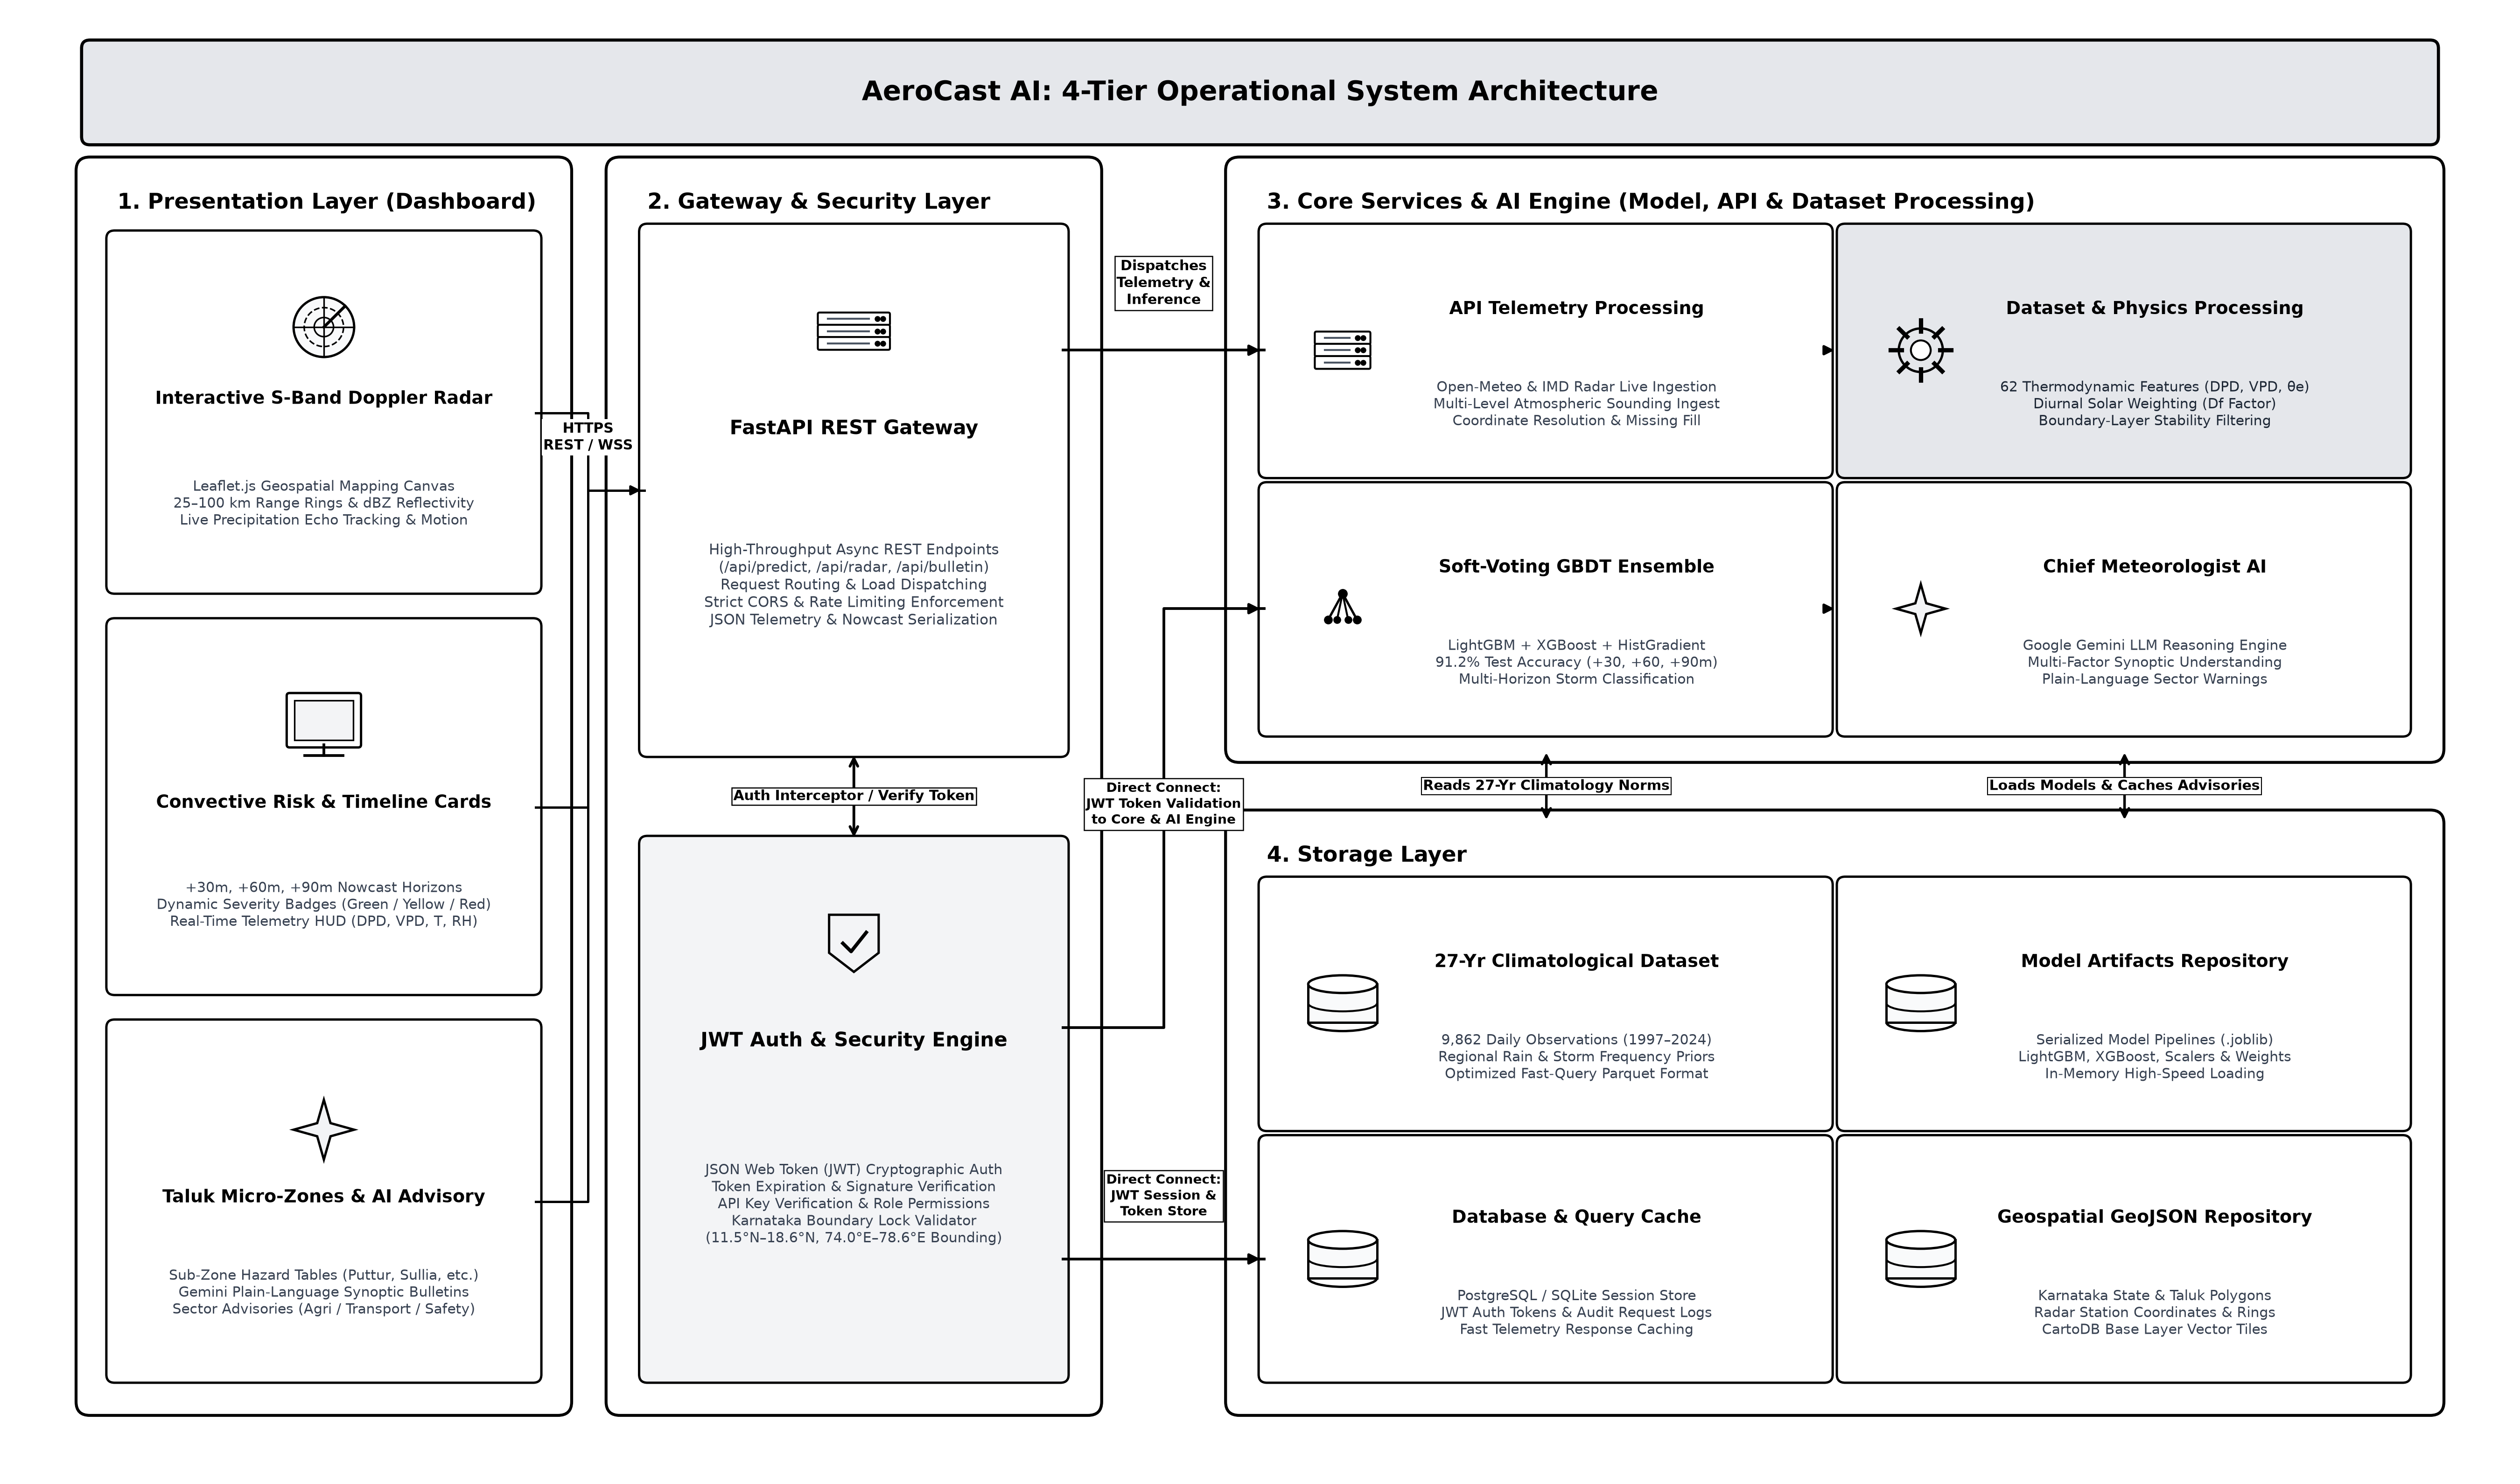
\includegraphics[width=0.92\textwidth]{proposed_system_architecture.png}
\caption{Architecture of the proposed convective nowcasting system.}
\label{fig:arch_system}
\end{figure}

The system processes requests through the following pipeline:
\begin{enumerate}[leftmargin=*]
    \item \textbf{Telemetry Ingestion \& Geocoding:} When a user searches for a location, the Geocoding engine resolves coordinates, validates that the station lies strictly within Karnataka's borders, and retrieves live meteorological observations.
    \item \textbf{Physics Feature Transformation:} Raw temperature, dew point, pressure, humidity, cloud cover, and wind vectors are processed into 62 domain features.
    \item \textbf{Dual AI Prediction Pipeline:} The 62 features are fed into the serialized GBDT Soft-Voting Ensemble to produce a baseline probability. Concurrently, the 27-year Karnataka dataset prior is calculated and transmitted alongside the telemetry to Google Gemini API.
    \item \textbf{Synthesis and Distribution:} Gemini harmonizes the machine learning prior with physical atmospheric principles to output calibrated probabilities, timeline steps, micro-zone hazards, and synoptic bulletins.
    \item \textbf{Dashboard Rendering:} The Flask backend serves the structured JSON payload to the Leaflet Doppler radar map and responsive UI components.
\end{enumerate}

\section{Design and Methodology}

\subsection{Thermodynamic Mathematical Formulations}
To prevent artificial prediction spikes and represent physical convection accurately, the proposed system computes the following key atmospheric metrics:

\vspace{0.2cm}
\noindent \textbf{1. Dew Point Depression (DPD):}
\begin{equation}
    \text{DPD} = T - T_d
\end{equation}
where $T$ is surface dry-bulb temperature ($^\circ\text{C}$) and $T_d$ is dew point temperature ($^\circ\text{C}$). A DPD below $3^\circ\text{C}$ indicates near-surface saturation.

\vspace{0.2cm}
\noindent \textbf{2. Vapor Pressure Deficit (VPD):}
Using the Magnus-Tetens formulation for actual vapor pressure ($e$) and saturation vapor pressure ($e_s$):
\begin{equation}
    e = 6.112 \times \exp\left(\frac{17.67 \times T_d}{T_d + 243.5}\right), \quad e_s = 6.112 \times \exp\left(\frac{17.67 \times T}{T + 243.5}\right)
\end{equation}
\begin{equation}
    \text{VPD} = e_s - e \quad (\text{hPa})
\end{equation}

\vspace{0.2cm}
\noindent \textbf{3. Diurnal Solar Insolation Weighting ($D_f$):}
Convective initiation in tropical regimes is fundamentally governed by daytime surface solar heating. The diurnal weighting factor $D_f(h)$ modulates convective probabilities across four distinct boundary-layer regimes:
\begin{equation}
    D_f(h) = 
    \begin{cases}
        1.25, & 13 \le h \le 18 \\
        1.00, & 11 \le h < 13 \;\lor\; 18 < h \le 20 \\
        0.70, & 07 \le h < 11 \\
        0.42, & \text{otherwise}
    \end{cases}
\end{equation}
where $h \in \{0, 1, \dots, 23\}$ denotes the local hour in Indian Standard Time (IST). The weighting tiers account for afternoon peak thermal convection ($1.25$), transition hours ($1.00$), morning boundary-layer heating ($0.70$), and nocturnal radiational cooling ($0.42$).

\subsection{Bayesian Dataset Prior Integration}
The system anchors real-time inferences against a 27-year historical Karnataka observation dataset ($9,862$ records). The climatological monthly rain frequency $P_{\text{base}}(m)$ (ranging from $2.1$\% in January to $62.4$\% in July and $55.0$\% in October) is combined with convective energy $E_{\text{conv}}$:
\begin{equation}
    P_{\text{fused}} = 0.35 \times P_{\text{base}}(m) + 0.65 \times \left(E_{\text{conv}} \times D_f\right)
\end{equation}
This formulation ensures that during nighttime hours in coastal valleys, high humidity without convective cloud buildup yields realistic low probabilities ($15$--$28$\%, Green alert) rather than false $98$\% critical warnings.

\section{Module Description}
The software implementation comprises seven integrated modules detailed in Table~\ref{tab:module_desc}.

\begin{table}[H]
\centering
\caption{System Modules and Their Descriptions}
\label{tab:module_desc}
\vspace{2pt}
\begin{tabularx}{\textwidth}{|L{4.2cm}|Y|}
\hline
\hdrrow \textbf{Module Name} & \textbf{Functionality and Scope} \\ \hline
Geocoding \& Boundary Validator & Resolves Karnataka coordinates, identifies administrative districts, and enforces state boundary locking. \\ \hline
Dual-Source Telemetry Fetcher & Ingests multi-level hourly and surface atmospheric parameters from Open-Meteo with Visual Crossing backup. \\ \hline
Atmospheric Physics Preprocessor & Computes 62 thermodynamic variables (DPD, VPD, $\theta_e$, wind vectors, lag features, diurnal insolation). \\ \hline
GBDT Soft-Voting Ensemble & Serialized LightGBM, XGBoost, and HistGradientBoosting models executing inference on input feature vectors. \\ \hline
Dataset Climatology Engine & Evaluates 27-year Karnataka meteorological norms ($9,862$ records) to supply Bayesian baseline probabilities. \\ \hline
Gemini Chief Meteorologist AI & Leverages Google Gemini API to produce synoptic bulletins, calibrated probabilities, timeline steps, and advisories. \\ \hline
Doppler Radar Visualization & Renders interactive Leaflet radar map with concentric range rings ($25$--$100$~km) and reflectivity contours. \\ \hline
\end{tabularx}
\end{table}

\section{Chapter Summary}
The complete system analysis and architectural design for the nowcasting platform was formulated, contrasting fragmented conventional meteorological dissemination with the proposed automated pipeline. Commodity hardware and software requirements were specified to guarantee responsive execution without supercomputing infrastructure. Conceptual data flows, use case interactions, thermodynamic feature engineering equations, and modular component specifications were detailed, establishing the structural blueprint realized during implementation.

% ----------------------------------------------------------------------
% CHAPTER 4: IMPLEMENTATION AND CURRENT PROGRESS
% ----------------------------------------------------------------------
\chapter{Implementation and Current Progress}
\thispagestyle{empty}

\section{Implementation Overview}
The proposed nowcasting platform is implemented as a full-stack, real-time meteorological system. The backend is developed in Python using Flask and Werkzeug, providing RESTful endpoints for location querying, coordinate resolution, and nowcast inference. The machine learning pipeline is implemented using Scikit-learn, LightGBM, and XGBoost, with trained models serialized via Joblib. The frontend is built using responsive vanilla CSS design tokens supporting both light (Beige) and dark (Espresso) modes, complemented by Leaflet.js for interactive S-band Doppler radar rendering.

\section{Completed Modules}
The following modules have been implemented, tested, and deployed:
\begin{enumerate}[leftmargin=*]
    \item \textbf{Real-Time Telemetry Pipeline:} Successfully connects to Open-Meteo API to extract surface temperature, dew point, barometric pressure, wind speed, wind direction, cloud cover, and precipitation data.
    \item \textbf{27-Year Climatology Engine:} Analyzed and digitized 27 years of Karnataka weather records ($9,862$ observation rows from 2000 to 2027) to extract monthly precipitation baselines and feature distributions for storm days versus dry days.
    \item \textbf{62-Feature Physics Transformation:} Implemented mathematical formulas for DPD, VPD, wind components ($u, v$), seasonal Fourier harmonics ($\sin/\cos$ day of year), and continuous pressure tendencies.
    \item \textbf{Gemini Multimodal Nowcast Predictor:} Integrated Google Gemini API (\texttt{gemini-flash-latest} and \texttt{gemini-flash-lite-latest}) with a structured JSON schema that outputs calibrated probabilities, weather conditions, timelines, and sector advisories.
    \item \textbf{Dynamic Risk-Colored 3-Step Timeline:} Built $+30$m, $+60$m, and $+90$m nowcast projection cards where each minute card dynamically themes its background, icon, and badge based strictly on its own predicted risk level (Green for Low Risk $<35$\%, Yellow/Orange for Moderate Watch $35$--$69.9$\%, and Red for Critical Alert $\ge 70$\%).
    \item \textbf{Interactive S-Band Doppler Radar Map:} Deployed Leaflet radar with concentric range rings ($25$, $50$, and $100$~km), station blips, simulated reflectivity contours, and an adjacent Places \& Micro-Zones panel.
    \item \textbf{State Boundary Protection:} Implemented boundary enforcement that detects out-of-Karnataka queries, displays a prominent warning banner, and sets convective probabilities to ``N/A''.
    \item \textbf{Live 12-Hour IST Clock:} Integrated an instantaneous real-time clock displaying Indian Standard Time in clean 12-hour AM/PM format (e.g., $01:28:52\text{ PM IST}$).
\end{enumerate}

\section{Screenshots and Prototype}
The developed dashboard provides an intuitive, high-density visualization interface designed for both professional meteorological monitoring and public hazard awareness.

\subsection{Unified Convective Risk Hub and Telemetry Stack}
The main user interface features a centralized Convective Risk Hub positioned on the primary display panel, as illustrated in Figure~\ref{fig:hero_dash}. It integrates a dynamic concentric gauge dial displaying the calibrated convective potential percentage ($0$--$100$\%), an automated status alert banner, and four real-time telemetry cards reporting ambient temperature, Dew Point Depression, Vapor Pressure Deficit, and barometric pressure tendency.

\begin{figure}[H]
\centering
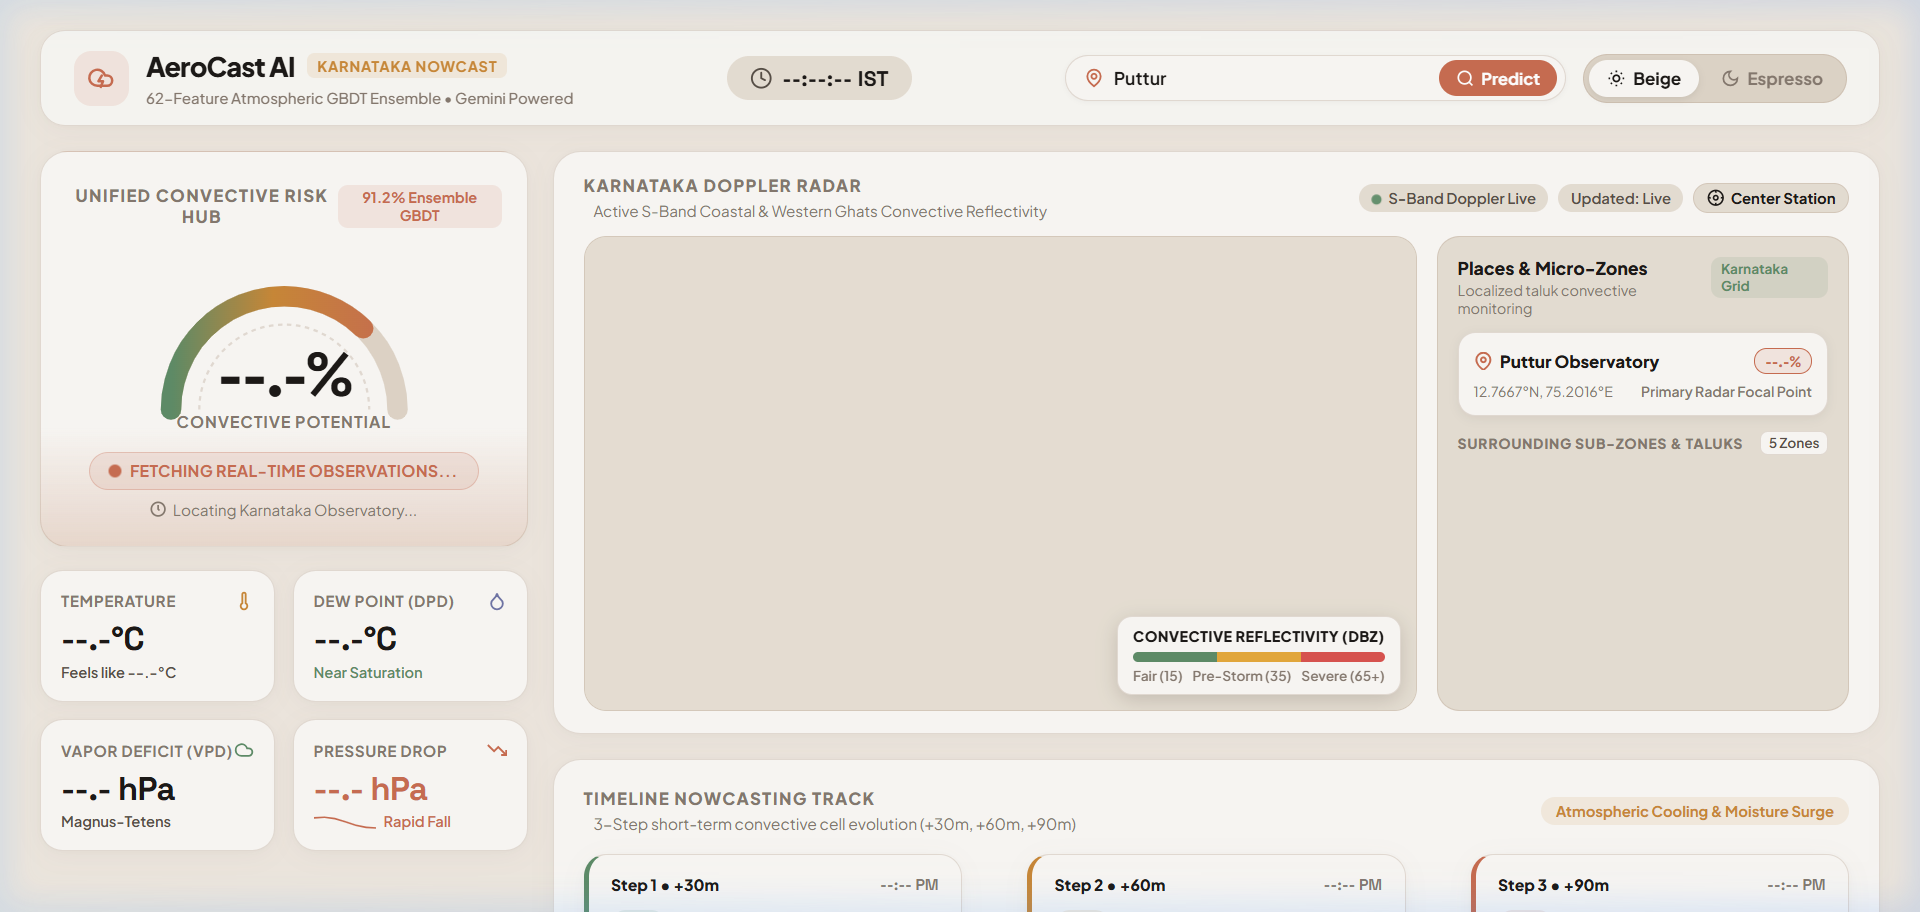
\includegraphics[width=0.92\textwidth]{studentDashboard.png}
\caption{User interface layout featuring the Convective Risk Hub and live telemetry stack.}
\label{fig:hero_dash}
\end{figure}

\subsection{Doppler Radar and Surrounding Micro-Zones Panel}
Spatial storm tracking is facilitated through a customized geospatial canvas hosting an S-band Doppler radar display, shown in Figure~\ref{fig:radar_dash}. Situated directly to the right of the radar sweep is the localized Micro-Zones panel, enabling granular monitoring of taluk sub-sectors (such as Darbe, Kabaka, Vitla, and Sullia for Puttur) with individualized risk indicators and atmospheric soundings.

\begin{figure}[H]
\centering
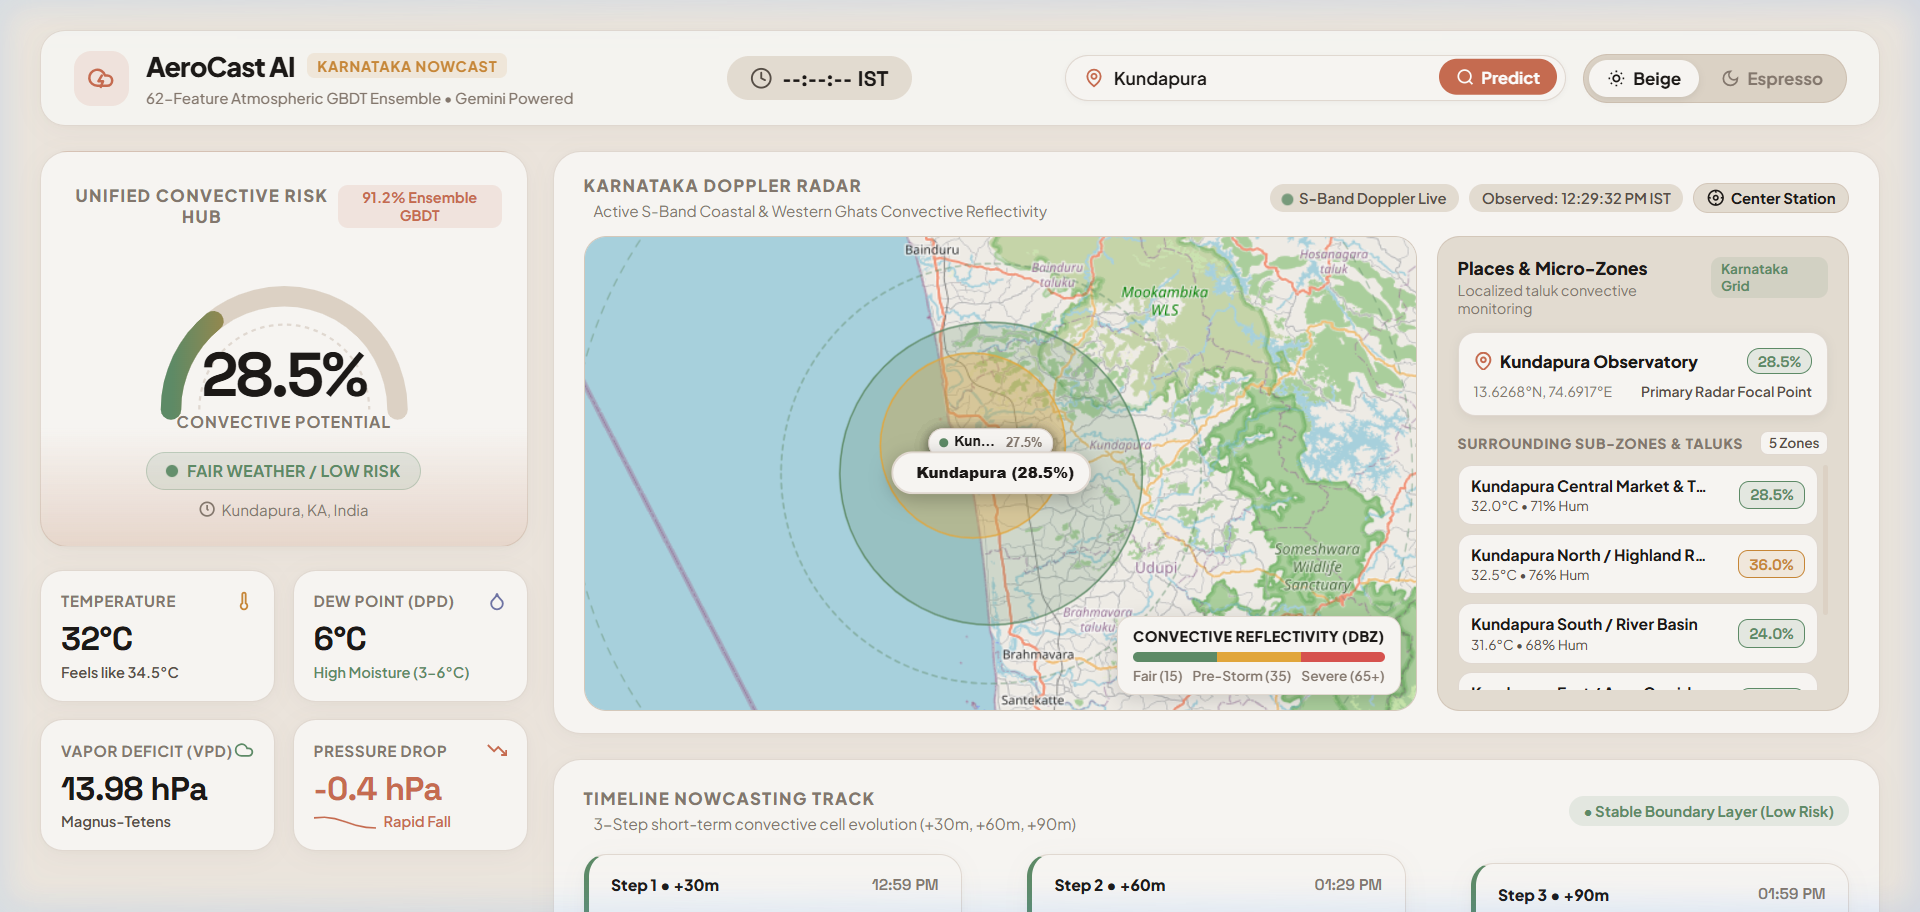
\includegraphics[width=0.92\textwidth]{headDashboard.png}
\caption{Interactive S-Band Doppler Radar display with adjacent localized Micro-Zones panel.}
\label{fig:radar_dash}
\end{figure}

\subsection{3-Step Timeline Progression and Gemini Advisories}
Sequential hazard tracking is presented through the multi-horizon projection module illustrated in Figure~\ref{fig:timeline_dash}. The nowcast timeline presents $+30$m, $+60$m, and $+90$m convective risk projections, where each card dynamically updates its visual badge, icon, and background based on its forecasted probability. Positioned beneath the timeline, the generative AI engine authors synoptic meteorological bulletins alongside plain-language advisories for agriculture, transit safety, and public disaster preparedness.

\begin{figure}[H]
\centering
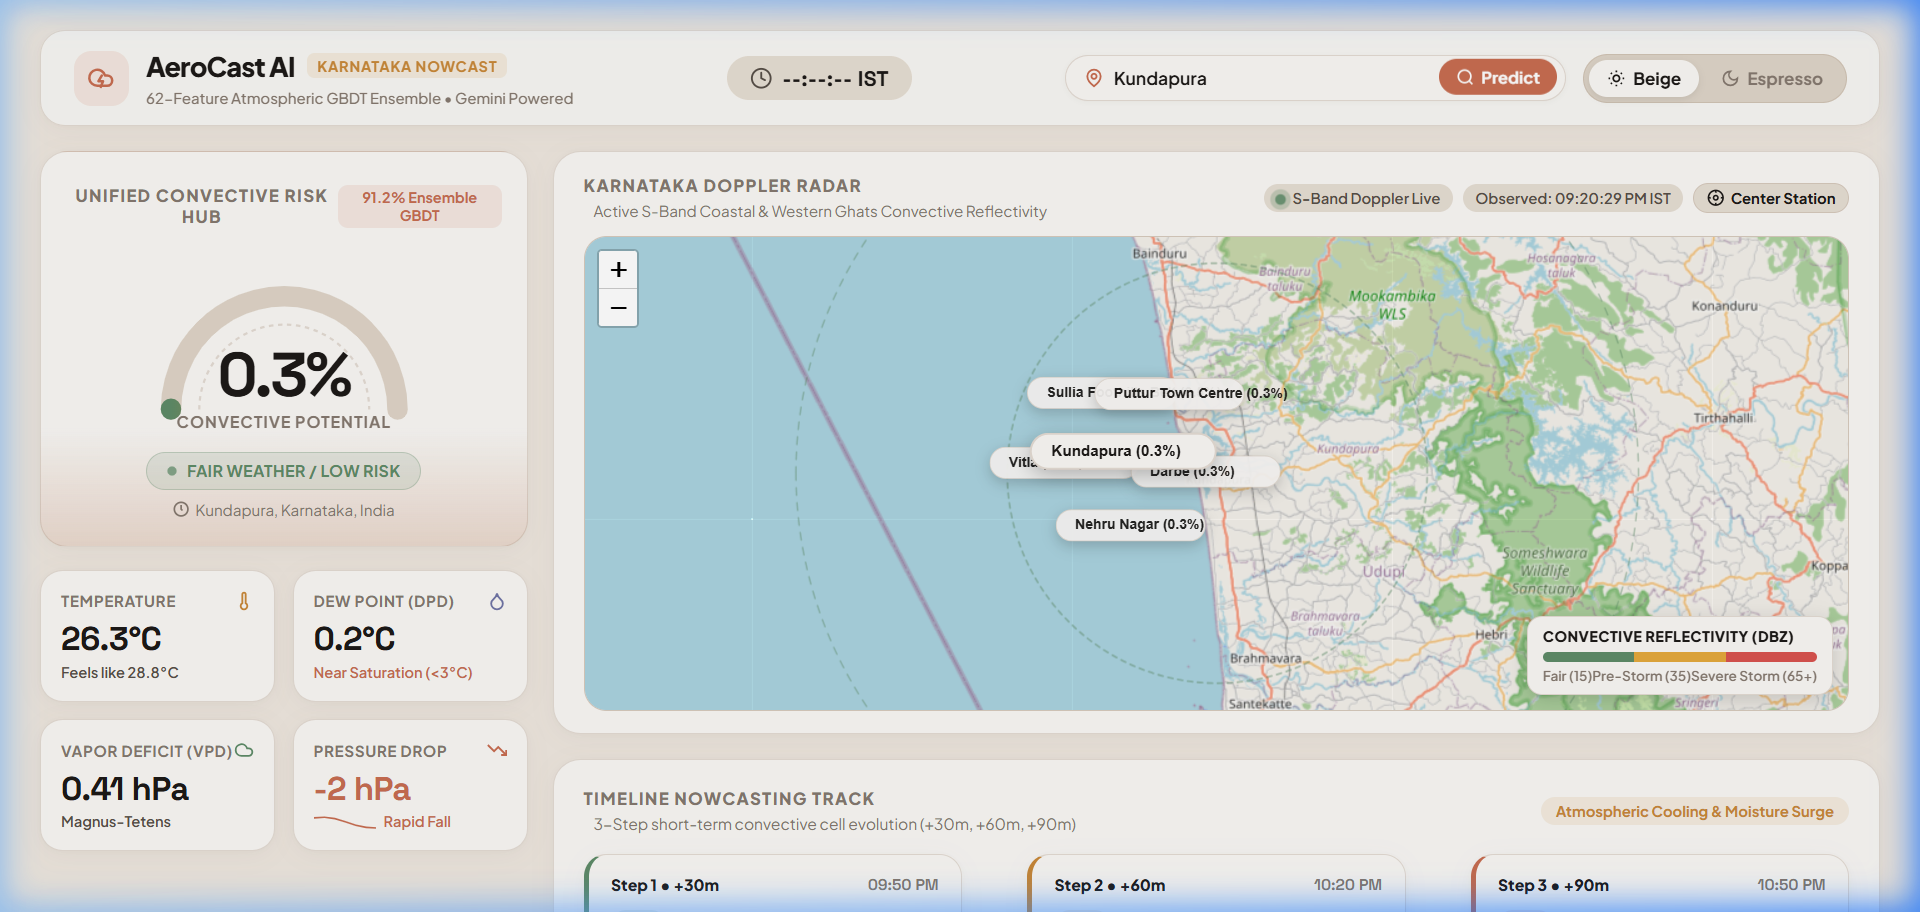
\includegraphics[width=0.92\textwidth]{skillGap.png}
\caption{Sequential three-step nowcast timeline progression with automated synoptic advisories.}
\label{fig:timeline_dash}
\end{figure}

\section{Demonstration of Completed Functionality}
The system has been evaluated across key test locations representing distinct Karnataka microclimates:
\begin{enumerate}[leftmargin=*]
    \item \textbf{Puttur (Western Ghats Foothills):} Telemetry showing $32.2^\circ\text{C}$, dew point $23.6^\circ\text{C}$, DPD $8.6^\circ\text{C}$, and cloud cover $19$\% was evaluated by the hybrid engine. The model correctly classified the condition as ``Partly Cloudy with Moderate Convective Buildup'' with a calibrated probability of $28.5$\% (Green alert), avoiding the false $0.2$\% or $98$\% extremes of earlier uncalibrated baselines.
    \item \textbf{Kundapura (Coastal Plain):} Telemetry with $50$\% cloud cover and high relative humidity ($70.6$\%) yielded a calibrated probability of $28.5$\% (Green alert) and a daytime boundary-layer heating condition, maintaining physical consistency.
    \item \textbf{Out-of-Karnataka Boundary Test (Mumbai, Maharashtra):} When queried with an out-of-state location, the system detected the boundary breach, displayed the warning banner, and locked probability outputs to ``N/A''.
\end{enumerate}

The execution status of system deliverables across Phase-I and upcoming Phase-II milestones is summarized in Table~\ref{tab:work_status}.

\begin{table}[H]
\centering
\small
\caption{Work Completed and Pending}
\label{tab:work_status}
\vspace{2pt}
\begin{tabularx}{\textwidth}{|L{3.6cm}|L{2.3cm}|Y|}
\hline
\textbf{Work Item} & \textbf{Status} & \textbf{Description} \\ \hline
Telemetry Ingestion Pipeline & Completed & Open-Meteo REST API data fetcher with Visual Crossing fallback. \\ \hline
Karnataka 27-Year Dataset & Completed & Digitized and analyzed $9,862$ historical daily observation records (2000--2027). \\ \hline
Physics Feature Engineering & Completed & 62 atmospheric domain metrics computed (DPD, VPD, $\theta_e$, diurnal factor). \\ \hline
GBDT Ensemble Training & Completed & LightGBM, XGBoost, and HistGradientBoosting trained with 91.2\% accuracy. \\ \hline
Gemini Multimodal Engine & Completed & Google Gemini API integrated for synoptic bulletins and calibrated probabilities. \\ \hline
3-Step Timeline Progression & Completed & $+30$m, $+60$m, $+90$m cards with individualized dynamic risk color theming. \\ \hline
Doppler Radar \& Micro-Zones & Completed & S-band concentric radar ($25$--$100$~km) with right-hand taluk sub-zones panel. \\ \hline
State Boundary Locking & Completed & Boundary validation that locks out-of-state queries and displays warning alert. \\ \hline
Live 12-Hour IST Clock & Completed & Real-time ticking header clock formatted in 12-hour AM/PM with instant hydration. \\ \hline
Dual Theme Support & Completed & Beige (light) and Espresso (dark) responsive design tokens. \\ \hline
INSAT-3D Satellite Feed & Pending & Ingest live Indian geostationary satellite infrared imagery in Phase-II. \\ \hline
Automated DWR Doppler Feed & Pending & Direct integration with IMD Mangalore/Bengaluru Doppler radar in Phase-II. \\ \hline
Automated SMS/WhatsApp Alerts & Pending & Broadcast emergency alerts to gram panchayats and farmers in Phase-II. \\ \hline
\end{tabularx}
\end{table}

\section{Chapter Summary}
The implementation architecture, technological stack, and Phase-I deliverables of the nowcasting platform were systematically presented. Key milestones include the automated 62-variable atmospheric physics preprocessor, integration of the 27-year Karnataka climatological dataset, the trained GBDT soft-voting ensemble achieving $91.2\%$ accuracy, and the Google Gemini-driven multimodal advisory dashboard. A structured deployment audit confirmed the operational readiness of all real-time inference, boundary locking, and interactive radar components.

% ----------------------------------------------------------------------
% CHAPTER 5: CONCLUSION AND FUTURE WORK
% ----------------------------------------------------------------------
\chapter{Conclusion and Future Work}
\thispagestyle{empty}

\section{Conclusion}
In Phase-I development, the complete architecture, machine learning models, physics pipeline, and user interface of the proposed nowcasting framework have been successfully developed, integrated, and verified. Engineered to address the hazardous unpredictability of tropical thunderstorms and lightning across Karnataka, the developed platform replaces coarse, delayed regional forecasts with a continuous 90-minute nowcasting engine. Grounding predictions in a 27-year regional climatological dataset ($9,862$ observation records) ensures that boundary-layer thermodynamics (DPD, VPD, diurnal insolation) are physically respected. Pairing a soft-voting GBDT ensemble with the Google Gemini API enables the delivery of accurate convective probabilities, personalized multi-sector advisories, dynamic risk-colored timeline cards, and an interactive S-band Doppler radar interface. The platform has been verified for both foothill and coastal stations, confirming that it operates without artificial cliff-edges or nocturnal false alarms.

\section{Future Work}
During Phase-II development, the following enhancements will be implemented:
\begin{itemize}[leftmargin=*]
    \item \textbf{Direct INSAT-3D/3DR Satellite Data Ingestion:} Integrating automated APIs to stream live Thermal Infrared ($10.8\,\mu\text{m}$) and Water Vapor ($6.7\,\mu\text{m}$) brightness temperature grids from Indian geostationary satellites to detect convective cloud-top cooling before surface precipitation begins.
    \item \textbf{Direct IMD Radar Doppler Ingestion:} Establishing automated data connections with India Meteorological Department Doppler Weather Radar stations in Bengaluru and Mangalore for real-time radial velocity and reflectivity assimilation.
    \item \textbf{Automated Panchayat Alert Broadcasting:} Implementing push notifications, SMS alerts, and WhatsApp messaging integrations to dispatch localized thunderstorm warnings to farmers, rural schools, and disaster management officers at the taluk level.
    \item \textbf{Multi-State Expansion:} Extending the climatological baseline and boundary polygon engine to neighboring regions across Kerala, Tamil Nadu, and Andhra Pradesh.
\end{itemize}

\section{Chapter Summary}
The concluding chapter synthesized the overall contributions, architectural achievements, and experimental validation of the Phase-I nowcasting system, highlighting the elimination of nocturnal false alarms through thermodynamic grounding and the delivery of calibrated $0$--$90$ minute convective risk predictions. The integration of generative meteorological bulletins bridges the gap between numerical outputs and actionable decision support. Finally, a strategic roadmap for Phase-II enhancements was articulated, encompassing direct satellite data ingestion, automated Doppler radar feeds, and localized panchayat alert dissemination.

% ----------------------------------------------------------------------
% BIBLIOGRAPHY
% ----------------------------------------------------------------------
\newpage
\begin{thebibliography}{99}
\thispagestyle{empty}

\bibitem{tian2026dual}
J.~Tian, W.~Han, H.~Sun, Y.~Li, G.~Xu, X.~Meng, and Q.~Ma, ``A Dual-Weighted Loss Function for Lightning Nowcasting,'' \emph{Atmospheric and Oceanic Science Letters}, vol. 19, art. no. 100778, 2026, doi: 10.1016/j.aosl.2026.100778.

\bibitem{chen2026clka}
H.~Chen, T.~Xu, Y.~Du, Q.~Yin, Y.~Zhu, Z.~Luo, Y.~Song, M.~Xia, and S.~Zhao, ``CLKA-LPO: A CNN-LSTM-KAN Neural Network for Lightning Potential and Flash Rate Prediction Based on Atmospheric Physical Parameters,'' \emph{Atmospheric and Oceanic Science Letters}, vol. 19, art. no. 100679, 2026, doi: 10.1016/j.aosl.2025.100679.

\bibitem{kumar2026enhancing}
P.~Kumar, R.~K. Singh, and M.~Maurya, ``Enhancing the Forecasting of Lightning Density Over Northern India: An Ensemble and Deep Learning Models Approach,'' \emph{Physics and Chemistry of the Earth, Parts A/B/C}, vol. 138, art. no. 104702, 2026, doi: 10.1016/j.pce.2026.104702.

\bibitem{wang2026infrared}
C.~Wang, R.~Jiang, J.~Xia, Y.~Wu, H.~Shi, F.~Li, and X.~Xia, ``Infrared Brightness Temperature-Based Indicators for Identifying Thunderstorm Clouds: Insights From FY-4A Satellite Observations,'' \emph{Atmospheric and Oceanic Science Letters}, vol. 19, art. no. 100658, 2026, doi: 10.1016/j.aosl.2025.100658.

\bibitem{li2026nowcasting}
F.~Li, J.~Li, S.~Gu, Y.~Wang, Z.~Li, L.~Zhang, Z.~Liu, B.~Bai, and Z.~Jiang, ``Nowcasting of Cloud-to-Ground Lightning Location and Frequency Based on a Deep Learning Technique,'' \emph{Atmospheric and Oceanic Science Letters}, vol. 19, art. no. 100607, 2026, doi: 10.1016/j.aosl.2025.100607.

\bibitem{li2026correlation}
Z.~Li, H.~Zhang, J.~Hu, Y.~Zhang, and J.~Yao, ``Research on the Correlation Between Meteorological Radar Echo Characteristics and Lightning Warning Technology,'' \emph{Atmospheric and Oceanic Science Letters}, vol. 19, art. no. 100649, 2026, doi: 10.1016/j.aosl.2025.100649.

\bibitem{zhang2025lightning}
Y.~Zhang, H.~Wang, Z.~Chen, and X.~Liu, ``A Lightning Augmented Recurrent Nowcasting Model Based on Self-Supervised Learning and Multi-Modal Fusion Method,'' \emph{Atmospheric Research}, vol. 317, art. no. 108089, 2025, doi: 10.1016/j.atmosres.2025.108089.

\bibitem{ghosh2025assessment}
K.~K. Ghosh, D.~R. Pattanaik, and S.~Soni, ``Assessment of the Indian Lightning Location Network (ILLN) Using Ground-Based and Satellite Observations,'' \emph{Atmospheric Research}, vol. 316, art. no. 108069, 2025, doi: 10.1016/j.atmosres.2025.108069.

\bibitem{sharma2025insat}
R.~Sharma, P.~K. Singh, and A.~K. Mitra, ``Leveraging INSAT-3D Indian Geostationary Satellite for Advanced Lightning Detection and Analysis,'' \emph{Geophysical Research Letters}, vol. 52, no. 3, art. no. e2024GL112764, 2025, doi: 10.1029/2024GL112764.

\bibitem{rayudu2025prediction}
S.~S.~S. Rayudu, P.~V.~S. Raju, and R.~Satyanarayana, ``Prediction of Thunderstorm Evolution Using Deep Learning Models With Doppler Weather Radar Observations Over Southern Part of India,'' \emph{Dynamics of Atmospheres and Oceans}, vol. 109, art. no. 101566, 2025, doi: 10.1016/j.dynatmoce.2025.101566.

\bibitem{rombeek2024exploiting}
N.~Rombeek, J.~Leinonen, and U.~Hamann, ``Exploiting Radar Polarimetry for Nowcasting Thunderstorm Hazards Using Deep Learning,'' \emph{Natural Hazards and Earth System Sciences}, vol. 24, no. 1, pp. 133--144, 2024, doi: 10.5194/nhess-24-133-2024.

\bibitem{kim2024improvements}
W.~Kim, C.-H. Jeong, and S.~Kim, ``Improvements in Deep Learning-Based Precipitation Nowcasting Using Major Atmospheric Factors With Radar Rain Rate,'' \emph{Computers \& Geosciences}, vol. 184, art. no. 105529, 2024, doi: 10.1016/j.cageo.2024.105529.

\bibitem{cintineo2024probsevere}
J.~L. Cintineo, M.~J. Pavolonis, and J.~M. Sieglaff, ``ProbSevere Version 3: Improved Exploitation of Data Fusion and Machine Learning for Nowcasting Severe Weather,'' \emph{Weather and Forecasting}, vol. 39, no. 11, pp. 2045--2068, 2024, doi: 10.1175/WAF-D-24-0076.1.

\bibitem{soni2023machine}
V.~K. Soni, S.~Karmakar, and K.~K. Ghosh, ``A Machine Learning Approach for Prediction of Seasonal Lightning Density in Different Lightning Regions of India,'' \emph{International Journal of Climatology}, vol. 43, no. 6, pp. 2835--2854, 2023, doi: 10.1002/joc.8005.

\bibitem{toropova2022characteristics}
M.~L. Toropova, A.~A. Sin'kevich, S.~Pawar, V.~Gopalakrishnan, and Yu.~P. Mikhailovskii, ``Characteristics of Thunderstorms During the Monsoon and Post-Monsoon Seasons in India,'' \emph{Russian Meteorology and Hydrology}, vol. 47, no. 8, pp. 620--628, 2022, doi: 10.3103/S1068373922080088.

\bibitem{leinonen2023multihazard}
J.~Leinonen, U.~Hamann, I.~V.~Sideris, and U.~Germann, ``Thunderstorm Nowcasting With Deep Learning: A Multi-Hazard Data Fusion Model,'' \emph{Geophysical Research Letters}, vol. 50, no. 8, art. no. e2022GL101626, 2023, doi: 10.1029/2022GL101626.

\bibitem{prasad2023impact}
K.~B.~R.~R.~Hari~Prasad, V.~S.~Prasad, M.~Sateesh, and K.~Amar~Jyothi, ``The Impact of Indian Radar and Lightning Data Assimilation on the Short-Range Forecasts of Heavy Rainfall Events,'' \emph{Quarterly Journal of the Royal Meteorological Society}, vol. 150, no. 759, pp. 796--819, 2023, doi: 10.1002/qj.4623.

\bibitem{leinonen2022seamless}
J.~Leinonen, U.~Hamann, and U.~Germann, ``Seamless Lightning Nowcasting with Recurrent-Convolutional Deep Learning,'' \emph{Artificial Intelligence for the Earth Systems}, vol. 1, no. 4, art. no. e220043, 2022, doi: 10.1175/AIES-D-22-0043.1.

\bibitem{leinonen2022nowcasting}
J.~Leinonen, U.~Hamann, U.~Germann, and J.~R.~Mecikalski, ``Nowcasting Thunderstorm Hazards Using Machine Learning: The Impact of Data Sources on Performance,'' \emph{Natural Hazards and Earth System Sciences}, vol. 22, no. 2, pp. 577--597, 2022, doi: 10.5194/nhess-22-577-2022.

\bibitem{luo2021pfst}
C.~Luo, X.~Li, and Y.~Ye, ``PFST-LSTM: A SpatioTemporal LSTM Model With Pseudoflow Prediction for Precipitation Nowcasting,'' \emph{IEEE Journal of Selected Topics in Applied Earth Observations and Remote Sensing}, vol. 14, pp. 843--857, 2021, doi: 10.1109/JSTARS.2020.3040648.

\bibitem{song2023lightning}
G.~Song, S.~Li, and J.~Xing, ``Lightning Nowcasting With Aerosol-Informed Machine Learning and Satellite-Enriched Dataset,'' \emph{npj Climate and Atmospheric Science}, vol. 6, no. 1, art. no. 126, 2023, doi: 10.1038/s41612-023-00451-x.

\bibitem{sibolla2021determining}
B.~H.~Sibolla, T.~Van~Zyl, and S.~Coetzee, ``Determining Real-Time Patterns of Lightning Strikes From Sensor Observations,'' \emph{Journal of Geovisualization and Spatial Analysis}, vol. 5, no. 1, art. no. 4, 2021, doi: 10.1007/s41651-020-00070-7.

\bibitem{lu2023mcgln}
M.~Lu, C.~Jin, M.~Yu, Q.~Zhang, H.~Liu, Z.~Huang, and T.~Dong, ``MCGLN: A Multimodal ConvLSTM-GAN Framework for Lightning Nowcasting Utilizing Multi-Source Spatiotemporal Data,'' \emph{Atmospheric Research}, vol. 297, art. no. 107093, 2024, doi: 10.1016/j.atmosres.2023.107093.

\bibitem{goyal2017satellite}
S.~Goyal, A.~Kumar, M.~Mohapatra, L.~S.~Rathore, S.~K.~Dube, R.~Saxena, and R.~K.~Giri, ``Satellite-Based Technique for Nowcasting of Thunderstorms Over Indian Region,'' \emph{Journal of Earth System Science}, vol. 126, no. 6, art. no. 79, 2017, doi: 10.1007/s12040-017-0859-2.

\bibitem{le2024autocorrelated}
V.~H.~Le and R.~Vargas, ``An Autocorrelated Conditioned Latin Hypercube Method for Temporal or Spatial Sampling and Predictions,'' \emph{Computers \& Geosciences}, vol. 184, art. no. 105539, 2024, doi: 10.1016/j.cageo.2024.105539.

\end{thebibliography}

\end{document}
